\chapter{Manipulación de bits}

Todos los datos en los programas de computadora se almacenan internamente como bits,
es decir, como números 0 y 1.
Este capítulo discute la representación de bits
de los enteros y muestra ejemplos
de cómo usar operaciones de bits.
Resulta que hay muchos usos para
la manipulación de bits en la programación de algoritmos.

\section{Representación de bits}

\index{representación de bits}

En la programación, un entero de $n$ bits se guarda internamente
como un número binario que consta de $n$ bits.
Por ejemplo, el tipo \texttt{int} en C++ es
un tipo de 32 bits, lo que significa que cada número \texttt{int}
consta de 32 bits.

Aquí está la representación de bits de
el número \texttt{int} 43: 
\[00000000000000000000000000101011\]
Los bits en la representación se indexan de derecha a izquierda.
Para convertir una representación de bits $b_k \cdots b_2 b_1 b_0$ en un número,
podemos usar la fórmula
\[b_k 2^k + \ldots + b_2 2^2 + b_1 2^1 + b_0 2^0.\]
Por ejemplo,
\[1 \cdot 2^5 + 1 \cdot 2^3 + 1 \cdot 2^1 + 1 \cdot 2^0 = 43.\]

La representación de bits de un número es
\key{con signo} o \key{sin signo}.
Por lo general, se utiliza una representación con signo,
lo que significa que se pueden representar
números negativos y positivos.
Una variable con signo de $n$ bits puede contener cualquier
entero entre $-2^{n-1}$ y $2^{n-1}-1$.
Por ejemplo, el tipo \texttt{int} en C++ es
un tipo con signo, por lo que una variable \texttt{int} puede contener cualquier
entero entre $-2^{31}$ y $2^{31}-1$.

El primer bit en una representación con signo
es el signo del número (0 para números no negativos
y 1 para números negativos) y
los $n-1$ bits restantes contienen la magnitud del número.
Se utiliza el \key{complemento a dos}, lo que significa que el
número opuesto de un número se calcula primero
invirtiendo todos los bits en el número,
y luego incrementando el número en uno.

Por ejemplo, la representación de bits de
el número \texttt{int} $-43$ es
\[11111111111111111111111111010101.\]

En una representación sin signo, solo se pueden usar
números no negativos, pero el límite superior para los valores es mayor.
Una variable sin signo de $n$ bits puede contener cualquier
entero entre $0$ y $2^n-1$.
Por ejemplo, en C++, una variable \texttt{unsigned int}
puede contener cualquier entero entre $0$ y $2^{32}-1$.

Existe una conexión entre las
representaciones:
un número con signo $-x$ es igual a un número sin signo $2^n-x$.
Por ejemplo, el siguiente código muestra que
el número con signo $x=-43$ es igual al número sin signo
$y=2^{32}-43$:
\begin{lstlisting}
int x = -43;
unsigned int y = x;
cout << x << "\n"; // -43
cout << y << "\n"; // 4294967253
\end{lstlisting}

Si un número es mayor que el límite superior
de la representación de bits, el número se desbordará.
En una representación con signo,
el siguiente número después de $2^{n-1}-1$ es $-2^{n-1}$,
y en una representación sin signo,
el siguiente número después de $2^n-1$ es $0$.
Por ejemplo, considere el siguiente código:
\begin{lstlisting}
int x = 2147483647
cout << x << "\n"; // 2147483647
x++;
cout << x << "\n"; // -2147483648
\end{lstlisting}

Inicialmente, el valor de $x$ es $2^{31}-1$.
Este es el valor más grande que se puede almacenar
en una variable \texttt{int},
entonces el siguiente número después de $2^{31}-1$ es $-2^{31}$.


\section{Operaciones de bits}

\newcommand\XOR{\mathbin{\char`\^}}

\subsubsection{Operación and}

\index{operación and}

La operación \key{and} $x$ \& $y$ produce un número
que tiene bits uno en las posiciones donde ambos
$x$ y $y$ tienen bits uno.
Por ejemplo, $22$ \& $26$ = 18, porque

\begin{center}
\begin{tabular}{rrr}
& 10110 & (22)\\
\& & 11010 & (26) \\
\hline
 = & 10010 & (18) \\
\end{tabular}
\end{center}

Usando la operación and, podemos verificar si un número
$x$ es par porque
$x$ \& $1$ = 0 si $x$ es par, y
$x$ \& $1$ = 1 si $x$ es impar.
Más en general, $x$ es divisible por $2^k$
exactamente cuando $x$ \& $(2^k-1)$ = 0.

\subsubsection{Operación or}

\index{operación or}

La operación \key{or} $x$ | $y$ produce un número
que tiene bits uno en posiciones donde al menos uno
de $x$ y $y$ tienen bits uno.
Por ejemplo, $22$ | $26$ = 30, porque


\begin{center}
\begin{tabular}{rrr}
& 10110 & (22)\\
$\XOR$ & 11010 & (26) \\
\hline
 = & 01100 & (12) \\
\end{tabular}
\end{center}

\subsubsection{Operación not}

\index{operación not}

La operación \key{not} \textasciitilde$x$
produce un número donde todos los bits de $x$
han sido invertidos.
La fórmula \textasciitilde$x = -x-1$ se mantiene,
por ejemplo, \textasciitilde$29 = -30$.

El resultado de la operación not a nivel de bit
depende de la longitud de la representación de bits,
porque la operación invierte todos los bits.
Por ejemplo, si los números son de 32 bits,
números \texttt{int}, el resultado es el siguiente:

\begin{center}
\begin{tabular}{rrrr}
$x$ & = & 29 &   00000000000000000000000000011101 \\
\textasciitilde$x$ & = & $-30$ & 11111111111111111111111111100010 \\
\end{tabular}
\end{center}

\subsubsection{Desplazamientos de bits}

\index{desplazamiento de bits}

El desplazamiento de bits a la izquierda $x < < k$ añade $k$
bits de cero al número,
y el desplazamiento de bits a la derecha $x > > k$
elimina los últimos $k$ bits del número.
Por ejemplo, $14 < < 2 = 56$,
porque $14$ y $56$ corresponden a 1110 y 111000.
De manera similar, $49 > > 3 = 6$,
porque $49$ y $6$ corresponden a 110001 y 110.

Tenga en cuenta que $x < < k$
corresponde a multiplicar $x$ por $2^k$,
y $x > > k$
corresponde a dividir $x$ por $2^k$
redondeado hacia abajo a un entero.

\subsubsection{Aplicaciones}

Un número de la forma $1 < < k$ tiene un bit de uno
en la posición $k$ y todos los demás bits son cero,
por lo que podemos usar tales números para acceder a bits individuales de los números.
En particular, el bit $k$ de un número es uno
exactamente cuando $x$ \& $(1 < < k)$ no es cero.
El siguiente código imprime la representación de bits
de un número \texttt{int} $x$:

\begin{lstlisting}
for (int i = 31; i >= 0; i--) {
    if (x&(1<<i)) cout << "1";
    else cout << "0";
}
\end{lstlisting}

También es posible modificar bits individuales
de números usando ideas similares.
Por ejemplo, la fórmula $x$ | $(1 < < k)$
establece el bit $k$ de $x$ en uno,
la fórmula
$x$ \& \textasciitilde $(1 < < k)$
establece el bit $k$ de $x$ en cero,
y la fórmula
$x$ $\XOR$ $(1 < < k)$
invierte el bit $k$ de $x$.

La fórmula $x$ \& $(x-1)$ establece el último
bit uno de $x$ a cero,
y la fórmula $x$ \& $-x$ establece todos los
bits uno a cero, excepto el último bit uno.
La fórmula $x$ | $(x-1)$
invierte todos los bits después del último bit uno.
Además, se debe tener en cuenta que un número positivo $x$ es
una potencia de dos exactamente cuando $x$ \& $(x-1) = 0$.

\subsubsection*{Funciones adicionales}

El compilador g++ proporciona las siguientes
funciones para contar bits:

\begin{itemize}
\item
$\texttt{\_\_builtin\_clz}(x)$:
la cantidad de ceros al principio del número
\item
$\texttt{\_\_builtin\_ctz}(x)$:
la cantidad de ceros al final del número
\item
$\texttt{\_\_builtin\_popcount}(x)$:
la cantidad de unos en el número
\item
$\texttt{\_\_builtin\_parity}(x)$:
la paridad (par o impar) de la cantidad de unos
\end{itemize}
\begin{samepage}

Las funciones se pueden utilizar de la siguiente manera:
\begin{lstlisting}
int x = 5328; // 00000000000000000001010011010000
cout << __builtin_clz(x) << "\n"; // 19
cout << __builtin_ctz(x) << "\n"; // 4
cout << __builtin_popcount(x) << "\n"; // 5
cout << __builtin_parity(x) << "\n"; // 1
\end{lstlisting}
\end{samepage}

\section{Representación de conjuntos}

Cada subconjunto de un conjunto
$\{0,1,2,\ldots,n-1\}$
se puede representar como un número entero de $n$ bits
cuyos bits uno indican qué
elementos pertenecen al subconjunto.
Esta es una forma eficiente de representar conjuntos,
porque cada elemento requiere solo un bit de memoria,
y las operaciones de conjuntos se pueden implementar como operaciones de bits.

Por ejemplo, dado que \texttt{int} es un tipo de 32 bits,
un número \texttt{int} puede representar cualquier subconjunto
del conjunto $\{0,1,2,\ldots,31\}$.
La representación de bits del conjunto $\{1,3,4,8\}$ es
\[00000000000000000000000100011010,\]
que corresponde al número $2^8+2^4+2^3+2^1=282$.

\subsubsection{Implementación de conjuntos}

El siguiente código declara una variable \texttt{int}
$x$ que puede contener
un subconjunto de $\{0,1,2,\ldots,31\}$.
Después de esto, el código agrega los elementos 1, 3, 4 y 8
al conjunto e imprime el tamaño del conjunto.
\begin{lstlisting}
int x = 0;
x |= (1<<1);
x |= (1<<3);
x |= (1<<4);
x |= (1<<8);
cout << __builtin_popcount(x) << "\n"; // 4
\end{lstlisting}
Luego, el siguiente código imprime todos
los elementos que pertenecen al conjunto:
\begin{lstlisting}
for (int i = 0; i < 32; i++) {
    if (x&(1<<i)) cout << i << " ";
}
// salida: 1 3 4 8
\end{lstlisting}

\subsubsection{Operaciones de conjuntos}

Las operaciones de conjuntos se pueden implementar como operaciones de bits de la siguiente manera:

\begin{center}
\begin{tabular}{lll}
& sintaxis de conjuntos & sintaxis de bits \\
\hline
intersección & $a \cap b$ & $a$ \& $b$ \\
unión & $a \cup b$ & $a$ | $b$ \\
complemento & $\bar a$ & \textasciitilde$a$ \\
diferencia & $a \setminus b$ & $a$ \& (\textasciitilde$b$) \\
\end{tabular}
\end{center}

Por ejemplo, el siguiente código primero construye
los conjuntos $x=\{1,3,4,8\}$ y $y=\{3,6,8,9\}$,
y luego construye el conjunto $z = x \cup y = \{1,3,4,6,8,9\}$:

\begin{lstlisting}
int x = (1<<1)|(1<<3)|(1<<4)|(1<<8);
int y = (1<<3)|(1<<6)|(1<<8)|(1<<9);
int z = x|y;
cout << __builtin_popcount(z) << "\n"; // 6
\end{lstlisting}

\subsubsection{Iteración a través de subconjuntos}

El siguiente código recorre
los subconjuntos de $\{0,1,\ldots,n-1\}$:

\begin{lstlisting}
for (int b = 0; b < (1<<n); b++) {
    // procesar subconjunto b
}
\end{lstlisting}
El siguiente código recorre
los subconjuntos con exactamente $k$ elementos:
\begin{lstlisting}
for (int b = 0; b < (1<<n); b++) {
    if (__builtin_popcount(b) == k) {
        // procesar subconjunto b
    }
}
\end{lstlisting}
El siguiente código recorre los subconjuntos
de un conjunto $x$:
\begin{lstlisting}
int b = 0;
do {
    // procesar subconjunto b
} while (b=(b-x)&x);
\end{lstlisting}

\section{Optimizaciones de bits}

Muchos algoritmos se pueden optimizar utilizando
operaciones de bits.
Estas optimizaciones no cambian la
complejidad del tiempo del algoritmo,
pero pueden tener un gran impacto
en el tiempo de ejecución real del código.
En esta sección discutimos ejemplos
de tales situaciones.

\subsubsection{Distancias de Hamming}

\index{Distancia de Hamming}
La \key{distancia de Hamming}
$\texttt{hamming}(a,b)$ entre dos
cadenas $a$ y $b$ de igual longitud es
el número de posiciones en las que las cadenas difieren.
Por ejemplo,
\[\texttt{hamming}(01101,11001)=2.\]

Considere el siguiente problema: Dado
una lista de $n$ cadenas de bits, cada una de longitud $k$,
calcule la distancia mínima de Hamming
entre dos cadenas en la lista.
Por ejemplo, la respuesta para $[00111,01101,11110]$
es 2, porque
\begin{itemize}[noitemsep]
\item $\texttt{hamming}(00111,01101)=2$,
\item $\texttt{hamming}(00111,11110)=3$, y
\item $\texttt{hamming}(01101,11110)=3$.
\end{itemize}

Una forma directa de resolver el problema es
recorrer todos los pares de cadenas y calcular
sus distancias de Hamming,
lo que produce un algoritmo de tiempo $O(n^2 k)$.
La siguiente función se puede utilizar para
calcular distancias:
\begin{lstlisting}
int hamming(string a, string b) {
    int d = 0;
    for (int i = 0; i < k; i++) {
        if (a[i] != b[i]) d++;
    }
    return d;
}
\end{lstlisting}

Sin embargo, si $k$ es pequeño, podemos optimizar el código
almacenando las cadenas de bits como enteros y
calculando las distancias de Hamming usando operaciones de bits.
En particular, si $k \le 32$, podemos almacenar
las cadenas como valores \texttt{int} y usar la
siguiente función para calcular distancias:
\begin{lstlisting}
int hamming(int a, int b) {
    return __builtin_popcount(a^b);
}
\end{lstlisting}
En la función anterior, la operación xor construye
una cadena de bits que tiene unos en posiciones
donde $a$ y $b$ difieren.
Luego, se calcula el número de bits usando
la función \texttt{\_\_builtin\_popcount}.

Para comparar las implementaciones, generamos
una lista de 10000 cadenas de bits aleatorias de longitud 30.
Usando el primer enfoque, la búsqueda tomó
13.5 segundos, y después de la optimización de bits,
sólo tomó 0.5 segundos.
Por lo tanto, el código optimizado de bits fue casi
30 veces más rápido que el código original.

\subsubsection{Contando subcuadrículas}

Como otro ejemplo, considere el
siguiente problema:
Dado una cuadrícula de $n \times n$ cuyo
cada cuadrado es negro (1) o blanco (0),
calcule el número de subcuadrículas
cuyas cuatro esquinas son negras.
Por ejemplo, la cuadrícula
\begin{center}
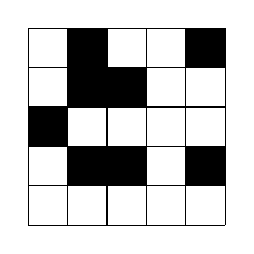
\begin{tikzpicture}[scale=0.5]
\fill[black] (1,1) rectangle (2,2);
\fill[black] (1,4) rectangle (2,5);
\fill[black] (4,1) rectangle (5,2);
\fill[black] (4,4) rectangle (5,5);
\fill[black] (1,3) rectangle (2,4);
\fill[black] (2,3) rectangle (3,4);
\fill[black] (2,1) rectangle (3,2);
\fill[black] (0,2) rectangle (1,3);
\draw (0,0) grid (5,5);
\end{tikzpicture}
\end{center}
contiene dos de estas subcuadrículas:
\begin{center}
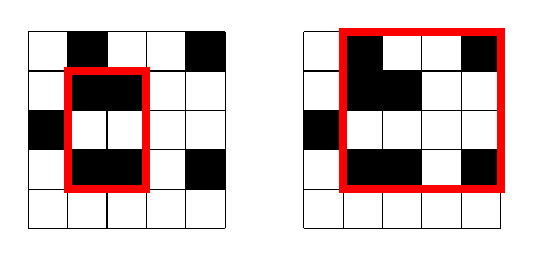
\begin{tikzpicture}[scale=0.5]
\fill[black] (1,1) rectangle (2,2);
\fill[black] (1,4) rectangle (2,5);
\fill[black] (4,1) rectangle (5,2);
\fill[black] (4,4) rectangle (5,5);
\fill[black] (1,3) rectangle (2,4);
\fill[black] (2,3) rectangle (3,4);
\fill[black] (2,1) rectangle (3,2);
\fill[black] (0,2) rectangle (1,3);
\draw (0,0) grid (5,5);

\fill[black] (7+1,1) rectangle (7+2,2);
\fill[black] (7+1,4) rectangle (7+2,5);
\fill[black] (7+4,1) rectangle (7+5,2);
\fill[black] (7+4,4) rectangle (7+5,5);
\fill[black] (7+1,3) rectangle (7+2,4);
\fill[black] (7+2,3) rectangle (7+3,4);
\fill[black] (7+2,1) rectangle (7+3,2);
\fill[black] (7+0,2) rectangle (7+1,3);
\draw (7+0,0) grid (7+5,5);

\draw[color=red,line width=1mm] (1,1) rectangle (3,4);
\draw[color=red,line width=1mm] (7+1,1) rectangle (7+5,5);
\end{tikzpicture}
\end{center}

Existe un algoritmo de tiempo $O(n^3)$ para resolver el problema:
recorre todos los $O(n^2)$ pares de filas y para cada par
$(a, b)$ calcula el número de columnas que contienen un cuadrado negro
en ambas filas en tiempo $O(n)$.
El siguiente código asume que $\texttt{color}[y][x]$
denota el color en la fila $y$ y columna $x$:
\begin{lstlisting}
int conteo = 0;
for (int i = 0; i < n; i++) {
    if (color[a][i] == 1 && color[b][i] == 1) conteo++;
}
\end{lstlisting}
Entonces, esas columnas
representan $\texttt{conteo}(\texttt{conteo}-1)/2$ subcuadrículas con esquinas negras,
porque podemos elegir cualquiera de los dos para formar una subcuadrícula.

Para optimizar este algoritmo, dividimos la cuadrícula en bloques
de columnas de tal manera que cada bloque consta de $N$
columnas consecutivas. Luego, cada fila se almacena como
una lista de números de $N$ bits que describen los colores
de los cuadrados. Ahora podemos procesar $N$ columnas al mismo tiempo
usando operaciones de bits. En el siguiente código,
$\texttt{color}[y][k]$ representa
un bloque de $N$ colores como bits.
\begin{lstlisting}
int conteo = 0;
for (int i = 0; i <= n/N; i++) {
    conteo += __builtin_popcount(color[a][i]&color[b][i]);
}
\end{lstlisting}
El algoritmo resultante funciona en tiempo $O(n^3/N)$.

Generamos una cuadrícula aleatoria de tamaño $2500 \times 2500$
y comparamos la implementación original y la optimizada con bits.
Mientras que el código original tardó $29.6$ segundos,
la versión optimizada con bits solo tardó $3.1$ segundos
con $N=32$ (números \texttt{int}) y $1.7$ segundos
con $N=64$ (números \texttt{long long}).

\section{Programación dinámica}

Las operaciones de bits proporcionan una forma eficiente y conveniente
de implementar algoritmos de programación dinámica
cuyos estados contienen subconjuntos de elementos,
porque tales estados se pueden almacenar como enteros.
A continuación, discutimos ejemplos de combinación
de operaciones de bits y programación dinámica.

\subsubsection{Selección óptima}

Como primer ejemplo, considere el siguiente problema:
Se nos dan los precios de $k$ productos
durante $n$ días, y queremos comprar cada producto
exactamente una vez.
Sin embargo, solo se nos permite comprar un producto como máximo
en un día.
¿Cuál es el precio total mínimo?
Por ejemplo, considere el siguiente escenario ($k=3$ y $n=8$):
\begin{center}
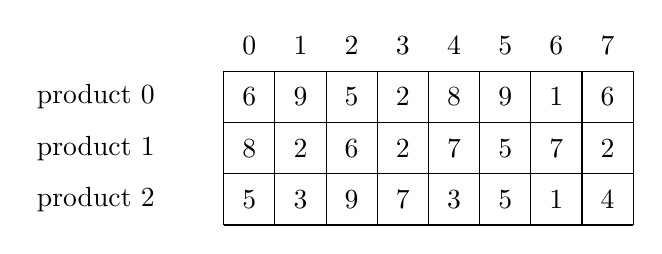
\begin{tikzpicture}[scale=.65]
    \draw (0, 0) grid (8,3);
    \node at (-2.5,2.5) {product 0};
    \node at (-2.5,1.5) {product 1};
    \node at (-2.5,0.5) {product 2};

    \foreach \x in {0,...,7}
        {\node at (\x+0.5,3.5) {\x};}
    \foreach \x/\v in {0/6,1/9,2/5,3/2,4/8,5/9,6/1,7/6}
        {\node at (\x+0.5,2.5) {\v};}
    \foreach \x/\v in {0/8,1/2,2/6,3/2,4/7,5/5,6/7,7/2}
        {\node at (\x+0.5,1.5) {\v};}
    \foreach \x/\v in {0/5,1/3,2/9,3/7,4/3,5/5,6/1,7/4}
        {\node at (\x+0.5,0.5) {\v};}
\end{tikzpicture}
\end{center}
En este escenario, el precio total mínimo es $5$:
\begin{center}
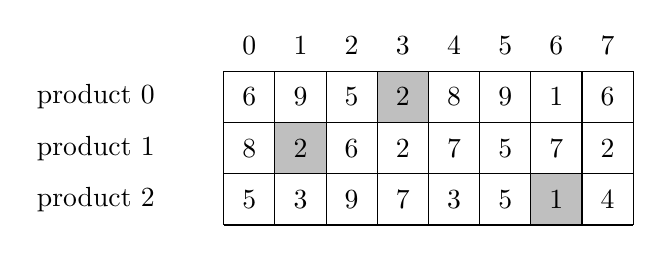
\begin{tikzpicture}[scale=.65]
    \fill [color=lightgray] (1, 1) rectangle (2, 2);
    \fill [color=lightgray] (3, 2) rectangle (4, 3);
    \fill [color=lightgray] (6, 0) rectangle (7, 1);
    \draw (0, 0) grid (8,3);
    \node at (-2.5,2.5) {product 0};
    \node at (-2.5,1.5) {product 1};
    \node at (-2.5,0.5) {product 2};

    \foreach \x in {0,...,7}
        {\node at (\x+0.5,3.5) {\x};}
    \foreach \x/\v in {0/6,1/9,2/5,3/2,4/8,5/9,6/1,7/6}
        {\node at (\x+0.5,2.5) {\v};}
    \foreach \x/\v in {0/8,1/2,2/6,3/2,4/7,5/5,6/7,7/2}
        {\node at (\x+0.5,1.5) {\v};}
    \foreach \x/\v in {0/5,1/3,2/9,3/7,4/3,5/5,6/1,7/4}
        {\node at (\x+0.5,0.5) {\v};}
\end{tikzpicture}
\end{center}

Deje que $\texttt{precio}[x][d]$ denote el precio del producto $x$
en el día $d$.
For example, in the above scenario $\texttt{price}[2][3] = 7$.
Then, let $\texttt{total}(S,d)$ denote the minimum total
price for buying a subset $S$ of products by day $d$.
Using this function, the solution to the problem is
$\texttt{total}(\{0 \ldots k-1\},n-1)$.

First, $\texttt{total}(\emptyset,d) = 0$,
because it does not cost anything to buy an empty set,
and $\texttt{total}(\{x\},0) = \texttt{price}[x][0]$,
because there is one way to buy one product on the first day.
Then, the following recurrence can be used:
\begin{equation*}
\begin{split}
\texttt{total}(S,d) = \min( & \texttt{total}(S,d-1), \\
& \min_{x \in S} (\texttt{total}(S \setminus x,d-1)+\texttt{price}[x][d]))
\end{split}
\end{equation*}
This means that we either do not buy any product on day $d$
or buy a product $x$ that belongs to $S$.
In the latter case, we remove $x$ from $S$ and add the
price of $x$ to the total price.

The next step is to calculate the values of the function
using dynamic programming.
To store the function values, we declare an array
\begin{lstlisting}
int total[1<<K][N];
\end{lstlisting}
where $K$ and $N$ are suitably large constants.
The first dimension of the array corresponds to a bit
representation of a subset.

First, the cases where $d=0$ can be processed as follows:
\begin{lstlisting}
for (int x = 0; x < k; x++) {
    total[1<<x][0] = price[x][0];
}
\end{lstlisting}
Then, the recurrence translates into the following code:
\begin{lstlisting}
for (int d = 1; d < n; d++) {
    for (int s = 0; s < (1<<k); s++) {
        total[s][d] = total[s][d-1];
        for (int x = 0; x < k; x++) {
            if (s&(1<<x)) {
                total[s][d] = min(total[s][d],
                                    total[s^(1<<x)][d-1]+price[x][d]);
            }
        }
    }
}
\end{lstlisting}
The time complexity of the algorithm is $O(n 2^k k)$.

\subsubsection{From permutations to subsets}

Using dynamic programming, it is often possible
to change an iteration over permutations into
an iteration over subsets\footnote{This technique was introduced in 1962
by M. Held and R. M. Karp \cite{hel62}.}.
The benefit of this is that
$n!$, the number of permutations,
is much larger than $2^n$, the number of subsets.
For example, if $n=20$, then
$n! \approx 2.4 \cdot 10^{18}$ and $2^n \approx 10^6$.
Thus, for certain values of $n$,
we can efficiently go through the subsets but not through the permutations.

As an example, consider the following problem:
There is an elevator with maximum weight $x$,
and $n$ people with known weights
who want to get from the ground floor
to the top floor.
What is the minimum number of rides needed
if the people enter the elevator in an optimal order?

For example, suppose that $x=10$, $n=5$
and the weights are as follows:
\begin{center}
\begin{tabular}{ll}
person & weight \\
\hline
0 & 2 \\
1 & 3 \\
2 & 3 \\
3 & 5 \\
4 & 6 \\
\end{tabular}
\end{center}
In this case, the minimum number of rides is 2.
One optimal order is $\{0,2,3,1,4\}$,
which partitions the people into two rides:
first $\{0,2,3\}$ (total weight 10),
and then $\{1,4\}$ (total weight 9).

The problem can be easily solved in $O(n! n)$ time
by testing all possible permutations of $n$ people.
However, we can use dynamic programming to get
a more efficient $O(2^n n)$ time algorithm.
The idea is to calculate for each subset of people
two values: the minimum number of rides needed and
the minimum weight of people who ride in the last group.

Let $\texttt{weight}[p]$ denote the weight of
person $p$.
We define two functions:
$\texttt{rides}(S)$ is the minimum number of
rides for a subset $S$,
and $\texttt{last}(S)$ is the minimum weight
of the last ride.
For example, in the above scenario
\[ \texttt{rides}(\{1,3,4\})=2 \hspace{10px} \textrm{and}
\hspace{10px} \texttt{last}(\{1,3,4\})=5,\]
because the optimal rides are $\{1,4\}$ and $\{3\}$,
and the second ride has weight 5.
Of course, our final goal is to calculate the value
of $\texttt{rides}(\{0 \ldots n-1\})$.

We can calculate the values
of the functions recursively and then apply
dynamic programming.
The idea is to go through all people
who belong to $S$ and optimally
choose the last person $p$ who enters the elevator.
Each such choice yields a subproblem
for a smaller subset of people.
If $\texttt{last}(S \setminus p)+\texttt{weight}[p] \le x$,
we can add $p$ to the last ride.
Otherwise, we have to reserve a new ride
that initially only contains $p$.

To implement dynamic programming,
we declare an array
\begin{lstlisting}
pair<int,int> best[1<<N];
\end{lstlisting}
that contains for each subset $S$
a pair $(\texttt{rides}(S),\texttt{last}(S))$.
We set the value for an empty group as follows:
\begin{lstlisting}
best[0] = {1,0};
\end{lstlisting}
Then, we can fill the array as follows:

\begin{lstlisting}
for (int s = 1; s < (1<<n); s++) {
    // initial value: n+1 rides are needed
    best[s] = {n+1,0};
    for (int p = 0; p < n; p++) {
        if (s&(1<<p)) {
            auto option = best[s^(1<<p)];
            if (option.second+weight[p] <= x) {
                // add p to an existing ride
                option.second += weight[p];
            } else {
                // reserve a new ride for p
                option.first++;
                option.second = weight[p];
            }
            best[s] = min(best[s], option);
        }
    }
}
\end{lstlisting}
Note that the above loop guarantees that
for any two subsets $S_1$ and $S_2$
such that $S_1 \subset S_2$, we process $S_1$ before $S_2$.
Thus, the dynamic programming values are calculated in the
correct order.

\subsubsection{Counting subsets}

Our last problem in this chapter is as follows:
Let $X=\{0 \ldots n-1\}$, and each subset $S \subset X$
is assigned an integer $\texttt{value}[S]$.
Our task is to calculate for each $S$
\[\texttt{sum}(S) = \sum_{A \subset S} \texttt{value}[A],\]
i.e., the sum of values of subsets of $S$.

For example, suppose that $n=3$ and the values are as follows:
\begin{multicols}{2}
\begin{itemize}
\item $\texttt{value}[\emptyset] = 3$
\item $\texttt{value}[\{0\}] = 1$
\item $\texttt{value}[\{1\}] = 4$
\item $\texttt{value}[\{0,1\}] = 5$
\item $\texttt{value}[\{2\}] = 5$
\item $\texttt{value}[\{0,2\}] = 1$
\item $\texttt{value}[\{1,2\}] = 3$
\item $\texttt{value}[\{0,1,2\}] = 3$
\end{itemize}
\end{multicols}
In this case, for example,
\begin{equation*}
\begin{split}
\texttt{sum}(\{0,2\}) &= \texttt{value}[\emptyset]+\texttt{value}[\{0\}]+\texttt{value}[\{2\}]+\texttt{value}[\{0,2\}] \\ 
                      &= 3 + 1 + 5 + 1 = 10.
\end{split}
\end{equation*}

Because there are a total of $2^n$ subsets,
one possible solution is to go through all
pairs of subsets in $O(2^{2n})$ time.
However, using dynamic programming, we
can solve the problem in $O(2^n n)$ time.
The idea is to focus on sums where the
elements that may be removed from $S$ are restricted.

Let $\texttt{partial}(S,k)$ denote the sum of
values of subsets of $S$ with the restriction
that only elements $0 \ldots k$
may be removed from $S$.
For example,
\[\texttt{partial}(\{0,2\},1)=\texttt{value}[\{2\}]+\texttt{value}[\{0,2\}],\]
because we may only remove elements $0 \ldots 1$.
We can calculate values of \texttt{sum} using
values of \texttt{partial}, because
\[\texttt{sum}(S) = \texttt{partial}(S,n-1).\]
The base cases for the function are
\[\texttt{partial}(S,-1)=\texttt{value}[S],\]
because in this case no elements can be removed from $S$.
Then, in the general case we can use the following recurrence:
\begin{equation*}
    \texttt{partial}(S,k) = \begin{cases}
               \texttt{partial}(S,k-1) & k \notin S \\
               \texttt{partial}(S,k-1) + \texttt{partial}(S \setminus \{k\},k-1) & k \in S
           \end{cases}
\end{equation*}
Here we focus on the element $k$.
If $k \in S$, we have two options: we may either keep $k$ in $S$
or remove it from $S$.

There is a particularly clever way to implement the
calculation of sums. We can declare an array
\begin{lstlisting}
int sum[1<<N];
\end{lstlisting}
that will contain the sum of each subset.
The array is initialized as follows:
\begin{lstlisting}
for (int s = 0; s < (1<<n); s++) {
    sum[s] = value[s];
}
\end{lstlisting}
Then, we can fill the array as follows:
\begin{lstlisting}
for (int k = 0; k < n; k++) {
    for (int s = 0; s < (1<<n); s++) {
        if (s&(1<<k)) sum[s] += sum[s^(1<<k)];
    }
}
\end{lstlisting}
This code calculates the values of $\texttt{partial}(S,k)$
for $k=0 \ldots n-1$ to the array \texttt{sum}.
Since $\texttt{partial}(S,k)$ is always based on
$\texttt{partial}(S,k-1)$, we can reuse the array
\texttt{sum}, which yields a very efficient implementation.
